\section{Lecture 2: Non-uniqueness due to sampling}

\subsection{Introduction}
In previous lecture, we used a-priori information for filling information between different samples. For example take a exponential signal $$x(t) = Ae^{\alpha t}$$ We can do a unique reconstruction by just doing two measurements and filling everything in between by using a priori information of $x(t)$. Here we will look at what happens when we don't have a-priori information for reconstruction. 

\subsection{Non-uniqueness due to lack of a-priori Information}

Let's sketch the reconstruction of $x(t)$ for two measurements $$x(t_{1})= Ae^{\alpha t_{1}}$$ $$x(t_{2})= Ae^{\alpha t_{2}}$$  and $t_{1}\neq t_{2}$. If we have a-priori form we can fill everything in between $t_{1} and t_{2}$ and elsewhere using that information (black line in Figure \ref{fig:nonunique}). Now suppose we know the same samples $x(t_{1})$ and $x(t_{2})$ and a-priori form is not given, then how we will proceed with reconstruction. The problem is not that there are no possibilities but that there are too many of them. Some of them are shown in Figure \ref{fig:nonunique} along with the reconstruction when the given form is exponential. 

\begin{figure}[ht]
\centering
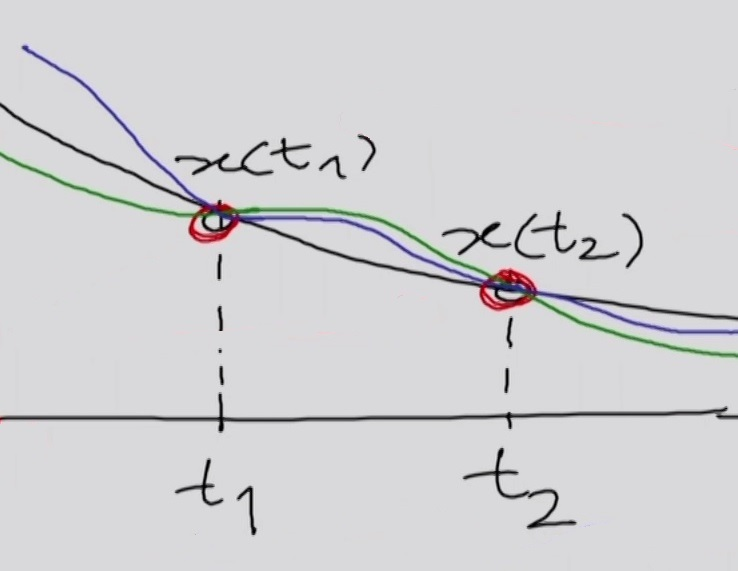
\includegraphics[width=0.7\textwidth]{nonunique.jpg}
\caption{\label{fig:nonunique}Non-unique reconstruction due to lack of a-priori Information}
\end{figure}

We can say the problem of sampling and reconstruction is similar to solving a crossword. We can think of clues as a-priori information and letters provided as samples.Without any a-priori information we can fill crossword any way we want but with clues we are restricted in our choice of filling up the crossword. Crosswords are generally designed such that there is a unique solution. Similarly in case of sampling and reconstruction a strong a-priori information restricts us to a unique reconstruction. 

\subsubsection{Degree of non-uniqueness in reconstruction}

When we know nothing about the form of signal then we see there is an infinity of possibilities. To answer how big is this infinity we must first see different classes of infinity. There is an infinity of natural numbers, infinity of integers, positive even/odd numbers etc. which are all same. Then there is an infinity of Real numbers which is bigger or higher than the infinity of integers in the sense that we can't put real numbers in one to one correspondence to integers without missing some real numbers. In case of reconstruction we need to define a value at every point. Some finite number of points have fixed value which are basically the samples but there is an infinity of points which don't have fixed value and can take any value in the absence of a-priori information. This infinity of possible reconstruction is thus even higher than infinity of real numbers. Now we can understand the degree of non-uniqueness of this problem.

How uniquely we can solve this problem of reconstruction depends on whether the given a-priori information completely complements the samples we have. We have previously seen that using Fourier transform we can represent a signal in terms of sinusoid. Let us take a sine wave and sample it and see what ambiguities we create. 

\subsection{Sampling Sinusoid}
Let us take a single sine wave and sample it uniformly i.e sampling with equal spacing between adjacent points. Now we need to find what are all sine waves which have these samples. The problem of ambiguity arises because we can miss an integer number of cycles between two samples. We can also arrive at a wrong edge. So with each possibility of losing a integer number of cycle one can also arrive at right edge or wrong edge. Let's analyse this mathematically bye taking $$A_{o}cos(\Omega _{o}t+\phi _{o})$$ as the form of sinusoid where $\Omega _{o}$ is the angular frequency and $T_{o}$ is the time period $$\Omega _{o}=\frac{2\pi }{T_{o}}$$ 

Now the process of sampling creates many 'ghost' or 'monster' frequencies which have the same samples at the same points. Let's denote these frequencies by $\Omega_{kj}$ where j($j = 1,2$) corresponds to two possibilities of correct or wrong edge. $$x(t) = A_{o}cos(\Omega _{kj}t+\phi _{kj})$$ $$k = 1,2,3,...$$ When $x(t)$ is sampled at time $nT_{s}$ where $n$ belongs to set of integers, we get $$x[nT_{s}]=A_{o}cos(\Omega _{o}nT_{s}+\phi _{o})$$ The non-uniqueness comes from being able to add a phase to this. Let's add $\pm 2\pi kn$ to the phase where $n$ is the sampling instant and $k$ belongs to set of positive integer. $$A_{o}cos(\Omega _{o}nT_{s}\pm 2\pi kn+\phi _{o})$$ $$=A_{o}cos(nT_{s}(\Omega _{o}\pm \frac{2\pi}{T_{s}}k)+\phi _{o})$$ $$=A_{o}cos(2 \pi nT_{s}(\frac{1}{T_{o}}\pm \frac{k}{T_{s}})+\phi _{o})$$ We need to have more than one sample in a cycle. We can see importance of this by taking a extreme example where we take just one sample per cycle and at the same location in every cycle. We will get same sample in every cycle. We cant even tell whether it is a DC or a sinusoid. Thus we can say that time interval between the samples must be less than cycle time.

$(\frac{1}{T_{o}}\pm \frac{k}{T_{s}})$ represents all possible Hertz frequencies. Let's take the possibility of $k=1$ $$(\frac{1}{T_{o}}-\frac{1}{T_{s}}) < 0$$ as $T_{s}<T_{o}$ but we don't want negative frequencies. Let's go back to original expression and see how we can correct this.$$A_{o}cos(2 \pi nT_{s}(\frac{1}{T_{o}}\pm \frac{k}{T_{s}})+\phi _{o})$$ $$=A_{o}cos\pm(2 \pi nT_{s}(\frac{1}{T_{o}}\pm \frac{k}{T_{s}})+\phi _{o})$$ If we take $+$ we get the same expression and if we take $-$ we get $$=A_{o}cos(-2 \pi nT_{s}(\mp\frac{k}{T_{s}}+ \frac{1}{T_{o}})-\phi _{o})$$ we see that the phase is reversed.

\subsubsection{Ghost Frequencies: An Example}
Let's take the case of $k=1$ again. Take $+$ for $(\frac{1}{T_{s}}+ \frac{1}{T_{o}})$ $$A_{o}cos(2 \pi nT_{s}(\frac{1}{T_{o}}+ \frac{1}{T_{s}})+\phi _{o})$$Take $-$ for $(-\frac{1}{T_{s}}+ \frac{1}{T_{o}})$ $$A_{o}cos(2 \pi nT_{s}(\frac{1}{T_{s}}- \frac{1}{T_{o}})-\phi _{o})$$

Take $T_{s}=\frac{T_{o}}{4}$ $$\frac{1}{T_{o}}+ \frac{1}{T_{s}} = \frac{5}{T_{o}}$$ $$\frac{1}{T_{s}}- \frac{1}{T_{o}} = \frac{3}{T_{o}}$$

Let's analyse this situation graphically. Take $T_{o}=\frac{\pi}{2}$
In Figure \ref{fig:sin} Black reconstruction is the true sinusoid and red is the sinusoid with ghost frequency $ = \frac{5}{T_{o}}$

\newpage

\begin{figure}[ht]
\centering
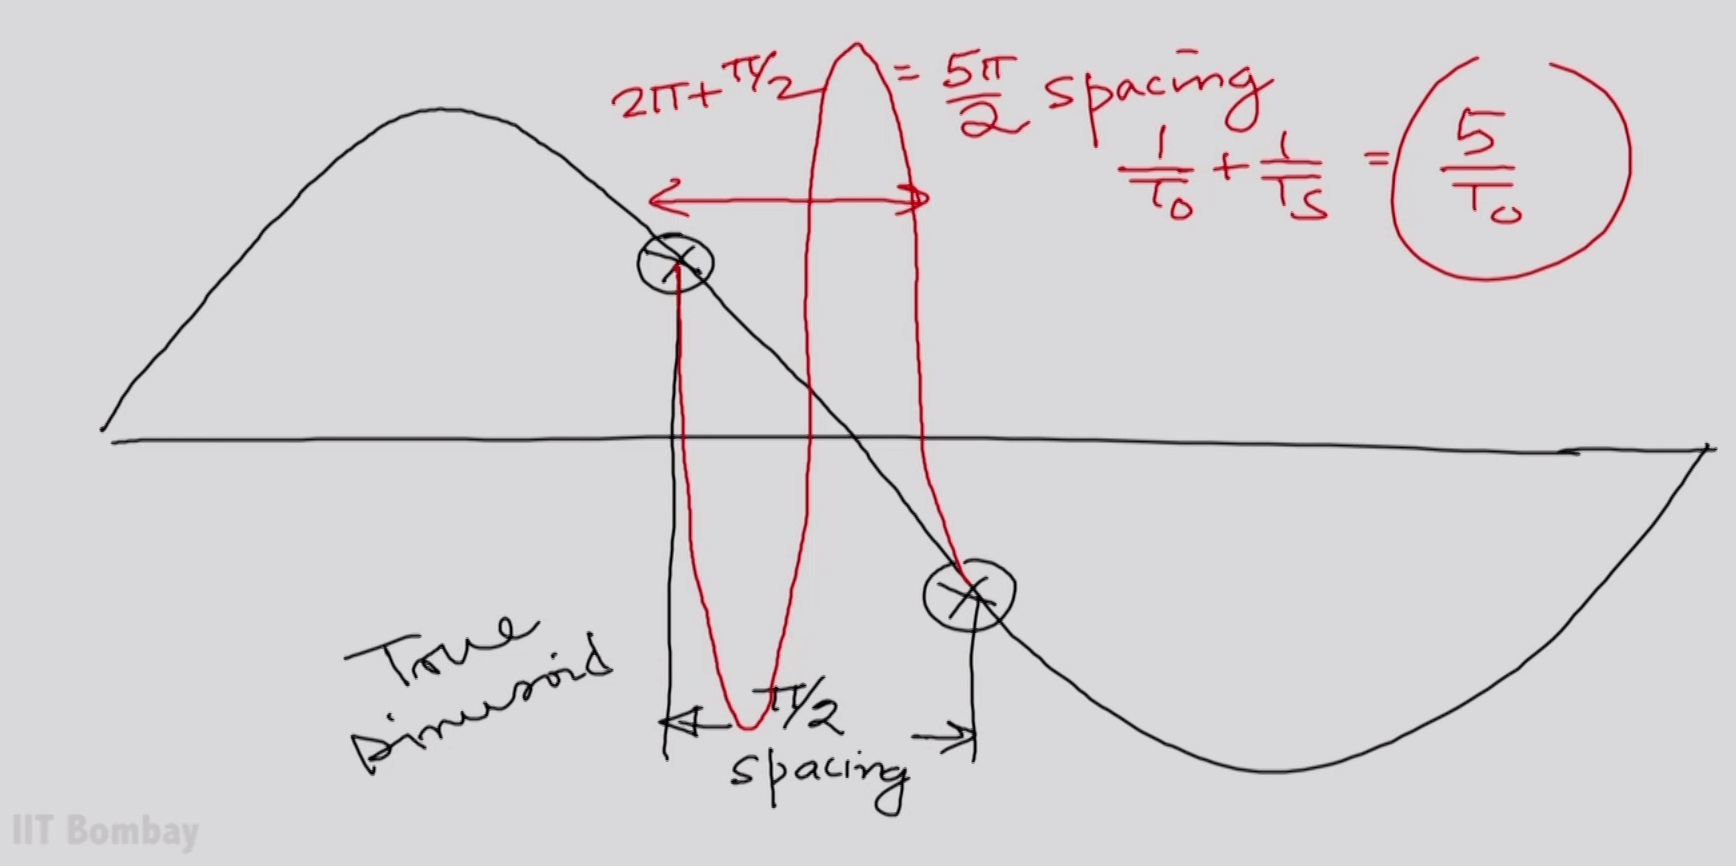
\includegraphics[width=1\textwidth]{sin.jpg}
\caption{\label{fig:sin}True sinusoid and Ghost frequencies}
\end{figure}

Exercise : Draw the sinusoid when you almost miss the cycle and arrive on the wrong edge and verify the ghost frequency $ = \frac{3}{T_{o}}$ and the spacing to be $\frac{3\pi}{2}$

